\section{Actor-Critic Methods}
\raggedbottom 
A wide range of reinforcement learning problems and many different approaches to effectively solve them exist.

Dynamic programming methods can compute optimal policies, however, a perfect model of the environment as MDP is required.

Monte-Carlo methods on the other hand can estimate value functions and discover optimal policies by averaging over sampled trajectories without a model.

\subsection{Monte-Carlo Predictions}

A complete run of the environment from start to termination is called an \textit{episode}.
Monte-Carlo methods require complete episodes to learn. They estimate the value of a state by calculating the discounted returns for every encountered state and changing the current estimate slightly in the direction of the discounted return.

MC-methods learn relatively fast, however each update requires a full episode.

\subsection{TD-Learning}

\citet{Sut98} describe \textit{temporal difference} (TD) learning as one of the central ideas in reinforcement learning.
TD learning combines dynamic programming and Monte-Carlo ideas to learn either \textit{state-values: V(s)} or \textit{state-action values: Q(s, a)}.
Like Monte-Carlo methods, TD methods can learn directly from experience without the need of a model, but do not require finished episodes. Instead the encountered rewards are combined with an estimate of the discounted return following them. This is called \textit{bootstrapping}.

We will take a look at the most basic TD method for learning a value function. 
The update step is given as:

\begin{equation}
V(s_t)\gets V(s_t)+ \alpha [r_{t+1} + \gamma V(s_{t+1})-V(s_t)]
\end{equation}

$\alpha$ denoted the learning rate.
Another popular TD-Method is Q-Learning.
It is used to estimate the state-action value function $Q$, and has a similar update step:

\begin{equation}
Q(s_t,a_t)\gets Q(s_t,a_t)+ \alpha [r_{t+1} + \gamma \max_a Q(s_{t+1},a)-Q(s_t,a_t)]
\end{equation}

After learning a Q-function, the agent has a reliable method to estimate and maximize the return, considering the learned function resembles the \textit{true state-value function} $Q*$ close enough. 
A common approach to achieve this is the use of a $\epsilon$-greedy policy, where a gradually decreasing value $\epsilon$ is used to decide if a random action or the action assumed to be the best according to the learned function is taken. 

This ensures both sufficient exploration and  exploitation, as it starts with a (mostly) random policy, and ends up with a deterministic policy always choosing the action with the highest estimated return \citep{Sut98}.

\begin{algorithm}[h]

 Initialize parameters for $Q(a,s)$ arbitrarily
 
 \Repeat{ training finished}
 { 
 Initialize s
 
 \Repeat{ s is terminal state}
 {
 
 Choose a from s using a policy derived from $Q$ (e.g. $\epsilon$ -greedy)
  
 Take action $a$, observe reward $r$ and next state $s'$
 $Q(s,a) \gets Q(s,a) + \alpha[r+ \gamma \max_{a'}Q(s',a')-Q(s,a)]$
 $s \gets s'$
 }
 }

 \caption{Q-Learning \citep{Sut98}}
\end{algorithm}


\subsection{N-Step TD-Learning}

The shown TD-Learning algorithms bootstrap after a single observation. This can become very inefficient with long episodes, especially if the final reward (e.g. winning or losing a game) is very important. Propagating this information along the trajectory requires many iterations.
In general, TD-Learning is rather slow compared to learning from full returns.

We can approach this problem by using n-step TD-learning.
Note that an '$ \infty $-step' TD update would be the same as a Monte-Carlo update.

By combining the Monte-Carlo target
\begin{equation}
R_t = r_{t+1}+\gamma r_{t+2}+\gamma^2 r_{t+3}+\gamma^3 r_{t+4}+ \dots +\gamma^{T-t-1} r_{T}
\end{equation}

 ($T$ denotes the final step of the episode) with the TD approach, we can define the n-step TD-learning update:
 
\begin{equation}
V(s_t) = V(s_t) + \alpha(\gamma^nV(s_{t+n})+R_{t:t+n} - V(s_t))
\end{equation} 

where 

\begin{equation}
R_{t:t+n} = r_{t+1}+\gamma r_{t+2}+\gamma^2 r_{t+3}+ \dots +\gamma^{n-1} r_{t+n}
\end{equation}

denotes the discounted return for the next n steps.
\subsection{Critic-Only Methods}

The shown Q-learning algorithm or SARSA are popular critic-only methods.

They do not contain an explicit function for the policy, but derive it from the learned state-action values by acting greedy on the Q-Values.

Critic-only methods provide a low variance estimate of the expected returns, however the methods suffer from being biased and can be problematic in terms of convergence.

\subsection{Actor-Only Methods}

Unlike critic-only methods, actor-only methods do not learn any state or state-action values.
Instead, they perform optimization steps directly on the policy $\pi$.

Usually the policy $\pi$ is parameterized by $\theta$, denoted as $\pi_\theta$, but deterministic policy gradient methods are possible \citep{DDPG}. 

Policy gradient methods like REINFORCE change the policy in order to maximize the average reward at a given timestep by performing gradient ascent \citep{Williams1992}. 
We define an objective function $J(\theta)$ which is a measurement of performance.

The learning agent tries to maximize $J(\theta)$ through gradient ascent

\begin{equation}
\theta_{t+1} = \theta_t + \alpha \widehat{\nabla J(\theta_t)}
\end{equation}

where $\widehat{\nabla J(\theta_t)}$ denotes an approximated gradient of the performance measure.
Methods of this schema are policy gradient methods \citep{Sut98}. 

For the episodic case we define $J(\theta)$ to be the initial value of our policy. We should note that this only works under the assumption, that the environments always provides the same initial state.

\begin{equation}
J(\theta) \doteq v_{\pi_\theta}(s_0)
\end{equation}

Because of the policy gradient theorem, the gradient of $J(\theta)$ , $ \nabla v_{\pi_\theta}(s_0)$ can be approximated as

\begin{equation}
\nabla J(\theta) \propto \sum_s \mu (s) \sum_a q_\pi (s,a) \nabla_\theta \pi(a \mid s, \theta).
\end{equation}

The proof for this theorem can be found in the reinforcement learning book by \citet{Sut98}.

$\mu$ denotes the on-policy distribution under $\pi$.

However, if trajectories are sampled on-policy, we can rewrite this as the expectation under policy $\pi$:

\begin{equation}
\nabla J(\theta) \propto E_\pi \left[ \sum_a q_\pi (s_t,a) \nabla_\theta \pi (a \mid s_t, \theta) \right]
\end{equation}


\begin{algorithm}[h]

 Initialize policy ($\pi$) parameters $\theta$ 
 
 \Repeat{forever}
 { 
 Generate episode: $s_0, a_0, r_1, \dots,s_{_{T-1}},   a_{_{T-1}}, r_{_T}$ following $\pi$ 
 
 \For { step $t \in{0,1,\dots, T}$}
 {
 $R \gets return from step t$
 
 $\theta \gets \theta + \alpha \gamma^t R\nabla_\theta ln(a_t \mid s_t, \theta)$
 }

 }

 \caption{REINFORCE by Williams \citep{Sut98}}
\end{algorithm}



In contrast to value based approaches, policy gradient methods provide strong convergence to at least a local maximum.
On top of that, actor methods are applicable on continuous action spaces
 \citep{Sutton00policygradient}.
 
Actor-only methods however suffer from a large variance of the gradient. Compared to critic-only methods their learning process is significantly slower \citep{Grondman12}.
 

\subsection{Actor-Critic Methods}

Actor-critic methods tackle the problem of high variance in policy gradient methods with the use of a critic.

They combine the strength of both approaches to achieve a learning agent, which has strong convergence, yet low variance.

Since actor-critic methods are still policy gradient methods at their core, they provide the possibility to work on continuous actions spaces like the actor-only approach.

The main reason for the variance in the gradient is the high variance of the return. By choosing a good baseline $ b(s)$, to the objective function, we can achieve a lower variance, without creating bias.
The idea behind this is to increase the probability of an action in relation to how much better it is compared to other actions at this state, rather than the full return.

\begin{equation}
\nabla J(\theta) \propto \sum_s \mu(s) \left[ \left( \sum_a q_\pi (s,a) -b(s)\right) \nabla_\theta \pi (a \mid s, \theta) \right]
\end{equation}

We can substitute $q_\pi(s_t,a) -b(s)$ with different terms \citep{Schulman15}.
Popular choices for actor-critic learning are the advantage function $A_\pi$ (\ref{adv}) or the TD residual 

\begin{equation}
r_t + V_\pi(s_{t+1}) - V_\pi(s_t)
\end{equation} 



\begin{figure}
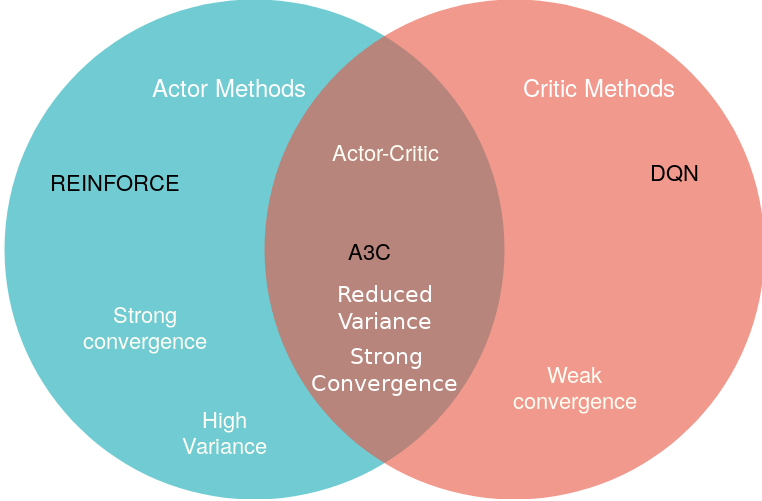
\includegraphics[scale=0.5]{bilder/actorcritic1.png}
\caption{Actor, Critic, and Actor-Critic approach}
\end{figure}

\pagebreak



\subsection{Asynchronous Advantage Actor Critic (A3C)}

In general we call an algorithm onpolicy, if the data used in the policy update was sampled under the same policy. The sequence of observed data encountered by an RL agent is strongly correlated and nonstationary \citep{A3C}. This can have a negative influence on the onpolicy learning process.

A previous approach to this problem was to achieve decorrelation by using randomly selected samples from a replay memory \citep{mnih2015atari}.

Training an agent comes with a high demand for computational power. To achieve feasible training times, former algorithms heavily relied on a strong GPU.

The asynchronous advantage actor critic (A3C) algorithm solves both problems, by training simultaneously on multiple environments.
Each learner samples trajectories and computes gradients. Those gradients are then applied to the shared parameters. 
After each global update step, the local parameters are synchronized.

This method not only enables efficient CPU computation with multiple threads, rather than requiring a strong GPU, but solves the problem of correlation since every environment can be assumed to be in different states.

Usually 16 or more environments are used to ensure proper decorrelation of the samples.

\pagebreak
A3C samples trajectories of length $n$ and uses the longest possible k-return for the update step, meaning the last state uses a one-step update, the second to last a two-step update and so on, with the first state using a n-step update.
The gradients are accumulated over all states within the trajectory and applied in a single gradient step. 

\begin{algorithm}[t]
// \textit{ Assume shared Parameters and counter} $ \theta^{global} ,\ \theta^{global}_v,\ T = 0 $

// \textit{ with local conterparts $\theta,\ \theta_v$}

 Initialize parameters for policy $\theta$ and critic $\theta_v$ and counter t=1
 
 \Repeat{T $ >$ T_{max}}
 { 
 Reset gradients $d\theta, d\theta_v$
 
 Synchronize $ \theta, \theta_v$ with $\theta^{global} ,\theta^{global}_v$
 
 t_{start} = t
 
 get state s_t

 \Repeat{$s_t$ \textbf{is} terminal or $(t - t_{start}) == t_{max}$}
 {
 
 \State Perform $a_t$ according to policy $\pi (a_t \mid s_t;\theta)$
 
 Receive reward $r_t$ and next state s_{t+1}
 
 $t \gets t + 1$
 
 $T \gets T + 1$

 }
 R = \begin{cases} 
 0 &  s_t \text{ terminal} \\
 V_{\theta}(s_t) & s_t \text{ not terminal}
 \end{cases} %]]>
 
 \For{ $i \in \{t -1,\dots, t_{start}\}$ }{
 $R \gets r_i + \gamma R$
 
 Accumulate gradients wrt. \theta : d\theta^{global} \leftarrow d\theta^{global} + \nabla_{\theta} \log \pi_{\theta’}(a_i \vert s_i)(R - V_{\theta_v}(s_i))
 
 Accumulate gradients wrt. \theta_v : d\theta^{global}_v \leftarrow d\theta^{global}_v + \partial (R - V_{\theta_v}(s_i))^2 / \partial \theta_v

 }
 Perform asynchronous update of $\theta^{global}$ and $\theta^{global}_v$ using d$\theta$, d$\theta_v$
 }

 \caption{A3C \citep{A3C}}
\end{algorithm}
